\subsection*{1}
    %Build a half-wave rectifier as shown below using a diode and resistor R = 33 k$\Omega$. Input
    %signal vs should be taken from the function generator. Use sinusoidal signal of frequency
    %100 Hz and amplitude about 2.5 V.

    A half-wave rectifier as shown in figure 1 below, was built using a  diode and r, R=33k$\Omega$.
    A sinusoidal signal of frequency 100 Hz and with a amplitude of about 2.5 V was used as the input signal, v$_s$.\\

    %FIG1 CIRCUIT DIAGRAM OF A HALFWAVE RECTIFIER
    \begin{figure}[h!]
        \centering
        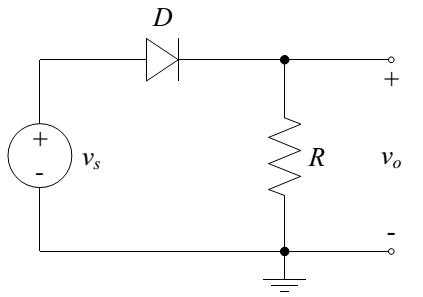
\includegraphics[width=5cm]{task1_1.png}
        \captionof{figure}{}
    \end{figure}

\subsection*{2}
    %Observe  the  input  signal  vs and  output  signal  vo using  the  oscilloscope.  
    %Determine  the voltage drop across the diode.

    The input signal, v$_s$, and the output signal, v$_o$, were observed using the oscilloscope and the voltage drop across the diode was determined.\\

    fig2%FIG2 OSCILLOSCOPE SHOWING INPUT AND OUTPUT SIFNALS

    Using values read from the oscilloscope seen in figure 2 above, the voltage drop across the diode was determined using the following formula.

    $$V_d = V_{s peak} - V_{o peak} = A\ V - B\ V = X\ V$$

\subsection*{3}
    %Modify the rectifier circuit as shown below:

    The half-wave rectifier circuit was modified by adding a capacitor C in parallel with resistor R as shown in figure 3 below.

    %FIG3 CIRCUIT DIAGRAM OF THE MODIFIED HALF-WAVE RECTIFIER
    \begin{figure}[h!]
        \centering
        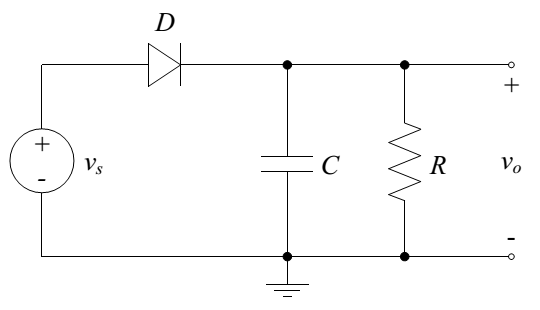
\includegraphics[width=6cm]{task1_3.png}
        \captionof{figure}{}
    \end{figure}

\subsection*{4}
    %For each of the following capacitance values C = 0.22 µF and C = 1 µF observe the input
    %and  output  signals  using  the  oscilloscope.  Determine  the  value  of  the  ripple  voltage  in
    %each case. 
    
    The input signal, v$_s$, and the output signal, v$_o$, were observed using the oscilloscope for the following capacitance values C = 0.22 $\mu$F and C = 1 $\mu$F and the ripple voltage was determined.\

\subsection*{5}
    %Compare  the  values  of  the  ripple  voltages  obtained  experimentally  with  the  theoretical
    %ones. 



